% Owned V123 contribution migrated to V130 evidence; numbers are generated by the V131 builder.
\section{Data collection and comparability}
\subsection{A traceable city--indicator matrix}
We compare $M=16$ cities on $N=10$ indicators covering safety, environment,
household costs, education and everyday resources. The initial matrix is the
team-supplied city table \cite{teamtable}. We retain its existing values, populations, reference
years and source flags as the agreed input, then supplement only empty cells.
Some supplied values lack original source URLs, so their provenance remains
the team table; official supplements do not retrospectively validate every
supplied measurement. Table~\ref{tab:indicators} states what each variable measures.

\begin{table}[htbp]\centering
\caption{Retained indicators, units and reference anchors. Supplied values are retained; supplements have explicit source scope.}\label{tab:indicators}
\begin{tabular}{p{.22\linewidth}p{.56\linewidth}r}
\toprule Indicator & Measurement and interpretation & Anchor\\\midrule
Homicide & Deaths per 100,000; cost; supplied city proxy & 2 \\
PM$_{2.5}$ & $\mu$g/m$^3$; cost; supplied concentration proxy & 15 \\
Living costs & Supplied living-cost index; cost & 100 \\
Housing & Supplied price-to-income ratio; cost & 10 \\
School resources & Pupils per teacher or explicitly scoped FTE; cost & 15 \\
Higher education & Institutions per 100,000; benefit; supply proxy & 1 \\
Transport stops & Unique stops per 100,000; benefit; partial inventories & 50 \\
Travel & Duration in minutes; $\exp(-t/30)$; commute or stage proxy & 30 min \\
Broadband & Supplied Mbps; benefit; city/general-use proxy & 100 \\
Swimming pools & Venues per 100,000; benefit; supply proxy & 1 \\
\bottomrule
\end{tabular}
\end{table}


The nominal reference year is 2025, but the evidence is mixed-vintage. Every
supplement retains its actual year rather than being relabelled as 2025.
Population denominators remain those of the supplied table. Thus a 2026 facility
snapshot divided by a supplied 2025 population is a conditional density, not an
observed same-year census. We do not infer that facilities are unchanged merely
because they may change slowly. Historical inventory assumptions are evaluated
through withdrawal scenarios.

We use official statistical tables, operator inventories and municipal geodata
to fill missing fields. For each admitted supplement, the archive records the
provider, URL, year, geographic and population scope, units, extraction rule and
file hash. Original PDFs and API responses are retained separately from derived
tables. Search summaries locate evidence; numerical admission requires the
underlying record or an explicitly identified provider capture. Values are
converted to compatible units before utility calculation: for example, the
supplied higher-education density per million is divided by ten to obtain the
per-100,000 scale. Mode share is not converted into physical stop density.

\subsection{Collection problems and their resolution}
\textbf{A station is not a platform, and a network is not a city.}
Oslo's municipal GIS represents platforms. Selecting records within the city
boundary and consolidating names gives 89 metro stations from 186 platforms.
Zurich's official 2025 VBZ report separately lists 446 stops on city territory
and 235 in the surrounding area; only 446 enter the city inventory
\cite{oslo,vbz}. A November 2026 snapshot of Helsinki's operator similarly
distinguishes 19 metro stations in Helsinki from 11 in Espoo \cite{helsinki}.
These are mode or operator subsets, so they supply
lower bounds rather than complete all-operator totals. For a verified facility
count $c$ and fixed population $P$, density is $d=10^5c/P$; utility is bounded by
$[d/(a+d),1]$.

Madrid's metro register contains 293 records. Of these, 242 carry code 28079 for the city, independently confirmed by INE. Omitting two unnamed records without lines and consolidating 240 named records by the provider's network-station identifier yields 191 city complexes. Linked multi-name complexes are conservatively counted once; 51 outside-city records are excluded \cite{madridmetro,inecodes}. This is a 29 May 2026 registered inventory with the supplied 2025 population, not a real-time operating count.

\textbf{A transport register can include non-passenger objects.}
Vienna's versioned operator files group stopping positions into DIVA station
areas. A broad route-pattern extraction yields 1,695 named city areas, but it
includes depot objects whose passenger-stop status is unproved. We reject that
count and retain 99 metro areas matched individually to the city's separate
existing-station layer and administrative polygon \cite{viennaogd,viennagis}.
Explicit spelling aliases are checked against both names and coordinates;
110 line appearances are not counted as 110 complexes. The 8 November 2026
export uses the unchanged supplied 2025 population. Its inventory membership
does not guarantee a departure or unrestricted access at a particular time.

Prague's current city-classified PID list supplies 57 named metro complexes
with route timetables \cite{pidmetro}. M\r{u}stek, Muzeum and Florenc each
count once despite two serving lines. The 2025 DPP report has 61 line
appearances and 58 distinct complexes; the current subset omits Flora,
whose 2026 closure is corroborated by the operator \cite{dpp2025,floraclose}.
Florenc's partial accessibility restriction does not close the whole complex.
Both supplements retain upper utility 1 for uncounted facilities.

Berlin's nine official U-Bahn route profiles contain 131 station appearances
in tariff zone A, defined by BVG as the Berlin inner city through the S-Bahn
ring. Native station identifiers consolidate these to 100 complexes; normalized
names are bijective with identifiers and cross-line transfers corroborate
repeated appearances \cite{bvg}. We retain this inner-city subset and leave
outer stations and other modes uncounted. The November 2026 published inventory
uses the supplied 2025 population; it measures registered resources rather
than real-time service or a student's individual access.

\textbf{A list of venues can contain closed facilities.}
Stockholm's current municipal swimming directory lists fourteen named venues,
one of which is explicitly closed for renovation. The thirteen retained venues
agree with the current overview; the temporary year-round replacement is
counted once \cite{stockpool}. We count venues, not individual basins. This
municipal subset gives a supply lower bound and leaves other providers unknown.
Its access date is November 2026; a page-footer date is not used to reconstruct
a 2025 inventory. Paris's 244 intra-muros metro stations come from a March 2022
atlas using RATP 2021 and Apur 2022 sources, not a 2025 observation
\cite{apur}. A separate withdrawal restores this historical supplement to unknown.

Tokyo's retained municipal subset consists of five indoor swimming venues at different Nerima addresses, verified against original city pages with 25-metre specifications. Heiwadai's current closure with no reopening date excludes it; Miharadai's announced February--May 2027 closure is distinguished from current stock \cite{nerimapool,nerimaclose}. Other wards/providers remain uncounted. The count measures venues, not lanes, basins or simultaneous opening.

\textbf{Pupils and teachers must refer to the same schools and stage.}
Prague's 2024/25 tables report 80,073 secondary-school pupils and 6,877.1
teacher full-time equivalents (FTE), including lower-gymnasium years.
Subtracting the matching 8,748 pupils and 737.8 FTE yields 71,325 pupils and
a rounding envelope of $[6139.2,6139.4]$ FTE \cite{prague}. The Prague
measure includes all study modes, including adult and non-daytime cohorts.
Stockholm's
published city-school ratio covers upper-secondary years 1--3 and all provider
ownership types, measured on 15 October \cite{kolada}. Its API value
16.42091405 is conservatively represented by $[16.35,16.45]$, an intentional
precision convention rather than a claimed measurement-error confidence interval.
For Henri-IV (Paris, UAI 0750654D), 2025 records give 794 lyc\'ee pupils
and 153.65 institution-level teacher FTE \cite{deppmatch}. FTEs lack an
upper-stage allocation; the 2026 directory flags post-baccalaureate provision
without recovering 2025 workloads \cite{deppdirectory}. Public/contracted-private
coverage also excludes other providers. These unmatched totals cannot identify
Paris's city PTR, which remains unknown. Dublin's payroll quality report states that school-roll FTE are not published; the available county or national aggregates cannot establish a matching city denominator \cite{irelandfte}.

\textbf{Unavailable records and unobserved travellers are retained honestly.}
An initial Singapore census PDF endpoint returned 404; the official Parliament
mirror and official data API supplied the report and matching table
\cite{singapore}. Duration bins are converted using utility at their endpoints,
without bin midpoints or an artificial maximum duration for the open tail.
The stage-specific total enrolment estimates exceed the travel-table estimates
by estimated uncovered student totals of 1,811 for secondary, 989 for
post-secondary non-tertiary and 1,635 for polytechnic. These are weighted
survey estimates rather than complete headcounts. The uncovered mass retains
utility $[0,1]$; unknown stage proportions are
handled by the interval convex hull. The resulting $[0.21048,0.61884]$ is a
2020 school-stage proxy, not an identified 2025 interval for ages 14--18.
When Dublin raw stop downloads returned 403, no count was inferred from the
catalogue. A later official map supported a separately documented subset of
19 existing city-centre tram stops \cite{dublin}. A timed-out Warsaw school-travel download
was discarded and the field left unknown. Failed retrieval does not create a
numerical observation.

The current 160 cells comprise 112 point values, 32 partial intervals and
16 fully missing intervals. The original table had 112 points, 12 partial
intervals and 36 fully missing cells. The twenty supplements therefore improve
information without replacing the team's existing measurements. Facility supply,
general commute proxies and school resources remain distinct from adolescent
access, school travel and learning quality.

\section{Establishing the baseline evaluation model}
\subsection{Determining indicator weights}
We retain eight main indicators at weight 0.1125 each and two auxiliary facility
indicators, transport stops and pools, at 0.05 each, so $\sum_jw_j=1$.
These weights express a transparent modelling choice. They are not estimated
from a student survey. Equal weights provide a separate reference.
TOPSIS is the primary score; VIKOR provides a focused method comparison.
AHP represents explicit preference scenarios \cite{saaty}, and Monte Carlo measures
sensitivity to declared distributions. These extensions retain the same
criteria rather than introduce unrelated ranking models.

For preference multipliers $m_j>0$, we use
\begin{equation}
 w'_j=\frac{m_jw_j}{\sum_kw_km_k},\qquad A_{jk}=\frac{w'_j}{w'_k}.
 \label{eq:weights}
\end{equation}
The principal eigenvector of $A$ recovers $w'$. With $\lambda_{\max}$ its
largest eigenvalue, $CI=(\lambda_{\max}-N)/(N-1)$ and $CR=CI/RI_N$.
Because this matrix is built from exact ratios, $\lambda_{\max}=N$ and
$CR=0$ up to numerical precision. This verifies internal consistency;
it does not establish that these are students' actual preferences.

\subsection{TOPSIS scoring calculation}
We adapt TOPSIS \cite{topsis} using fixed reference anchors to preserve a common scoring scale across evidence,
preference and future scenarios. For benefit and cost measurements respectively,
\begin{equation}
 u^{+}(x)=\frac{x}{a+x},\qquad u^{-}(x)=\frac{a}{a+x}.
\end{equation}
Each anchor in Table~\ref{tab:indicators} is a declared reference scale, not
an estimated optimum. Travel uses $q(t)=e^{-t/30}$ for duration $t$ in minutes.
When only mean duration $\bar t$ is known, Jensen's inequality gives
$\mathbb E[q(t)]\in[e^{-\bar t/30},1]$. Fully missing utilities remain $[0,1]$.

For utility vector $u_i$, weighted distances from fixed worst and best points are
\begin{equation}
 D_i^-=\sqrt{\sum_jw_ju_{ij}^2},\qquad
 D_i^+=\sqrt{\sum_jw_j(1-u_{ij})^2},\qquad
 S_i=100\frac{D_i^-}{D_i^-+D_i^+}.
\end{equation}
Weights enter the squared distances once. Since $S_i$ increases with every
utility, endpoints $\ell_i,h_i$ give $L_i=S(\ell_i)$ and $U_i=S(h_i)$.
Under the retained rectangular uncertainty set, define
\begin{equation}
 R_i=\max\{0,\max_{k\ne i}U_k-L_i\},\qquad
 i^*\in\arg\min_iR_i,
 \label{eq:regret}
\end{equation}
\begin{equation}
 \mathcal C=\{i:U_i\geq\max_{k\ne i}L_k\}.
\end{equation}
Maximum regret $R_i$ measures how far the selected city could trail another
city. Set $\mathcal C$ retains every city that could still be first.
The maximum excludes the selected city itself. These conditional data bounds
are not sampling confidence intervals, and a conservative recommendation does
not identify a uniquely best city.

\subsection{Scoring results and interpretation}
Zurich minimizes maximum regret, followed by Singapore and Oslo
(Table~\ref{tab:baseline}). Zurich's score lower bound is below those of
Singapore and Oslo; its own upper bound is excluded from its competitor set.
Its regret is $70.90353-53.53548=17.36805$, whereas Oslo's is
$72.18379-54.29594=17.88785$. All sixteen cities remain possible champions.
The decision order expresses a conservative recommendation under the stated
criteria and intervals.

\begin{table}[htbp]\centering
\caption{Conservative baseline decision ranks with unchanged weights.}\label{tab:baseline}
\begin{tabular}{rlrr}\toprule
Rank & City & Score interval & Maximum regret\\\midrule
1 & Zurich & 53.54--72.18 & 17.37 \\
2 & Singapore & 54.33--63.53 & 17.85 \\
3 & Oslo & 54.30--63.90 & 17.89 \\
4 & Stockholm & 52.12--64.54 & 20.06 \\
5 & Prague & 51.97--62.78 & 20.21 \\
6 & Dublin & 51.13--70.90 & 21.05 \\
7 & Berlin & 50.73--61.54 & 21.45 \\
8 & Helsinki & 49.41--69.84 & 22.78 \\
9 & Paris & 49.11--69.04 & 23.08 \\
10 & Madrid & 49.00--68.22 & 23.18 \\
11 & Vienna & 47.52--61.03 & 24.66 \\
12 & Warsaw & 47.50--63.99 & 24.69 \\
13 & Milan & 45.63--65.99 & 26.56 \\
14 & London & 45.17--66.12 & 27.01 \\
15 & Tokyo & 43.96--61.12 & 28.22 \\
16 & Amsterdam & 42.29--60.43 & 29.90 \\
\bottomrule\end{tabular}\end{table}




Holding weights and formulas fixed, the twenty admitted supplements narrow
the average fixed-weight score interval from 18.81077 to \CurrentMeanWidth{}, a
\TotalWidthReduction\% reduction. \LatestEvidenceChange
Earlier additions improved Stockholm's decision position. Withdrawal of the historical Paris and Dublin transport inventories still recommends Zurich; withdrawal of Singapore's historical school-stage travel proxy also preserves this recommendation. Evidence improves precision and changes decisions before it
necessarily reduces the possible-champion set.

As a method diagnostic, TOPSIS and VIKOR use the same illustrative midpoint
utilities and weights. VIKOR balances total and largest weighted shortfalls
equally and uses sample best/worst values \cite{vikor}. \MethodComparison
The midpoint comparison does not replace the interval decision in
Equation~\ref{eq:regret}. Agreement indicates similarity within the chosen
conventions; disagreement exposes method dependence rather than justifying a
post-hoc choice of the preferred winner.

\begin{figure}[!ht]
\centering
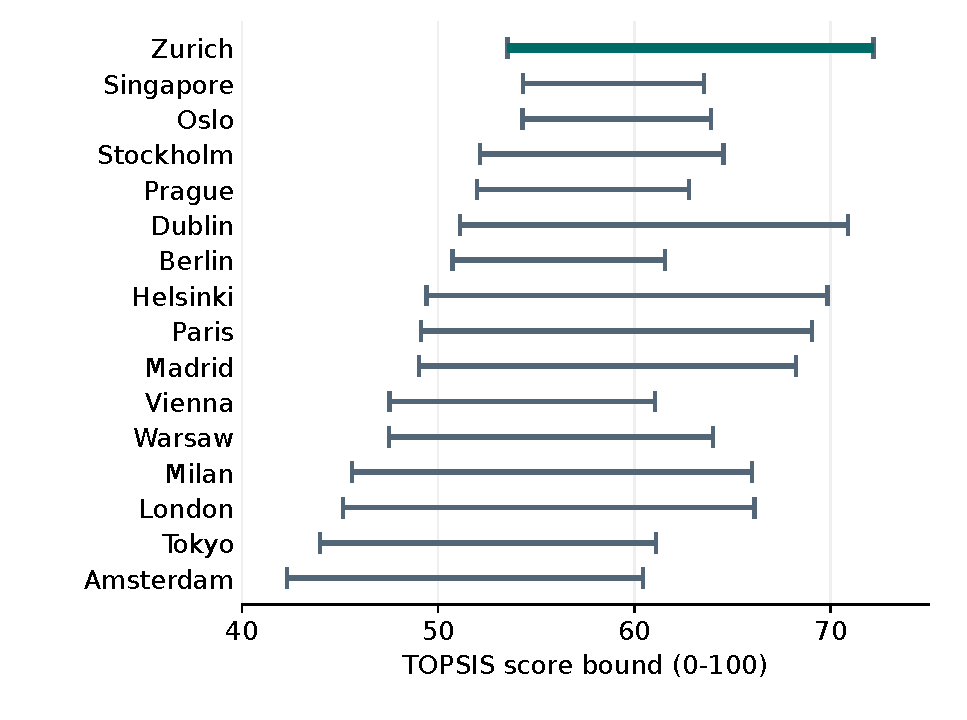
\includegraphics[width=\linewidth]{task4_v131_assets/score_intervals.pdf}
\caption{Current score bounds and conservative decision order for the sixteen
cities. Intervals retain missing information; they are not confidence intervals.
Source: frozen city matrix and admitted supplements.}
\label{fig:intervals}
\end{figure}

\FloatBarrier
\subsection{A significant revision: retaining uncertain evidence}
A controlled comparison shows why evidence bounds belong in the decision.
On the same 160 utility entries, compare the midpoint completion $z_{ij}=(\ell_{ij}+h_{ij})/2$ with the retained-interval formulation in Equation~\ref{eq:regret}. Both use identical weights, anchors and TOPSIS scores. The midpoint is a declared diagnostic scenario, rather than an estimate of missing observations or a reconstruction of the team's historical first model.

The revision retains 48 non-point entries and selects the city with the smallest worst-case shortfall. Zurich remains the recommendation, but 13 cities change decision rank under fixed weights; Kendall's $\tau_b=0.583$. With equal weights, 15 ranks change and $\tau_b=0.650$.

A constructed interior completion keeps other cities at their utility midpoints and sets every uncertain Zurich utility to $\ell_{ij}+0.1(h_{ij}-\ell_{ij})$. All 112 point values stay fixed, and all 48 uncertain values are strictly inside their intervals. Dublin scores 62.31483 and Zurich 55.54326, putting Zurich at decision position 13 in that completion. At adverse rectangular endpoints, Dublin's 70.90353 exceeds Zurich's 53.53548 by 17.36805, realizing Zurich's model maximum regret. Some endpoints represent raw-scale suprema; these constructions concern the declared utility rectangle, rather than an observed population or proof of joint physical attainability.

This revision separates a conditional first place from a conservative action while preserving all sixteen possible champions. It changes the handling of uncertainty within one score. The \TotalWidthReduction\% interval-width reduction comes separately from admitted data, not from this controlled formulation comparison.


\section{Model revision and extension}
\subsection{Considering future changes}
We examine three conditional changes while holding anchors and population
denominators fixed. Resource expansion raises higher-education, stop and pool
densities by 10\%. Living pressure raises living costs, housing cost ratios and
travel durations by 10\%. Balanced improvement reduces pupil--teacher ratios,
PM$_{2.5}$ and travel durations by 10\%. A comparable multi-year panel is not
available, so these changes have no estimated annual rate or forecast date.

For raw multiplier $r>0$, the utility transformations are
\begin{equation}
 T_r^{+}(u)=\frac{ru}{1-u+ru},\qquad
 T_r^{-}(u)=\frac{u}{u+r(1-u)}.
\end{equation}
These increasing maps propagate raw-scale changes through benefit and cost
intervals. For known mean travel duration, the new Jensen interval is
$[e^{-r\bar t/30},1]$. Singapore instead has bounds $[L_q,U_q]$ on expected
utility. With $q=e^{-t/30}$ and $t'=rt$, Jensen and $0\leq q\leq1$ give
\begin{equation}
 \mathbb E[q^r]\in
 \begin{cases}
 [L_q,U_q^r],&0<r<1,\\
 [L_q,U_q],&r=1,\\
 [L_q^r,U_q],&r>1.
 \end{cases}
 \label{eq:moment}
\end{equation}
Raising both endpoints to $r$ would generally misrepresent an expected utility.
Equation~\ref{eq:moment} is an outer moment bound and need not be reversible.
Fully missing travel remains unknown. Thus the extension accommodates the
different information supplied by means and by travel distributions.

\FutureDeterministic
We also solve a decision boundary: holding other cities fixed, proportionally
reduce one city's pupil--teacher ratio, PM$_{2.5}$ and travel durations until
its maximum regret ties that of the best other city. \FutureThresholds
These thresholds describe the model response to a specified joint change;
they do not establish policy feasibility or a uniquely identified champion.
\BerlinThresholdChange

For a separate future-shock simulation, each draw combines a common shock and
city-specific shocks under a declared bounded distribution, with the criterion
weights held fixed. Original data intervals are not randomly completed.
\FutureMonteCarlo
\ProxyWithdrawalMC
These are conditional stress frequencies under an uncalibrated distribution.
Weight perturbations below answer a separate question and are not blended
silently into the future-shock frequencies.

\subsection{Considering different preferences and development situations}
Education priority doubles the weights of the two education indicators.
The independent living scenario doubles travel and transport-stop weights.
Equation~\ref{eq:weights} then normalizes all weights.
\PreferenceResults
\PreferenceEvidenceChange
The resulting differences show how the definition of a desirable city affects
the decision. They do not establish measured differences between fourteen- and
eighteen-year-old students.

\subsection{Perturbing weights}
For each preference centre $w'$, we draw
$w^{(b)}\sim\operatorname{Dirichlet}(\kappa w')$, with
$\kappa\in\{20,100,500\}$ and 10,000 draws per setting. Every draw recomputes
interval TOPSIS and maximum regret without filling missing values. We report
mean decision rank, fractional first-place recommendation frequency and
fractional top-three decision membership; ties share membership.

\begin{table}[htbp]\centering
\caption{Conditional recommendation frequencies (\%) for selected cities at concentration 100.}
\begin{tabular}{lrrr}\toprule
Preference centre & Zurich & Oslo & Singapore\\\midrule
Baseline & 43.33 & 27.92 & 28.23 \\
Education priority & 6.83 & 42.95 & 41.43 \\
Independent living & 58.99 & 15.46 & 25.12 \\
\bottomrule\end{tabular}\end{table}




\MonteCarloInterpretation
These two summaries optimize different quantities. We retain minimum maximum
regret as the predeclared decision rule; Monte Carlo reports its sensitivity.
Neither average ranks nor a network aggregation resolves the missing empirical
information. A low AHP consistency ratio and repeated simulations demonstrate
calculation properties, not representative student opinion.

\subsection{Within-city fairness and growth stages}
Citywide facilities per resident measure supply, not who can use it. Fees,
opening hours, transport links, disability access and neighbourhood location
can separate nominal supply from student opportunity. Without matched student
locations and qualifying facilities, the city-level matrix cannot identify
these access distributions.

\EquityCase
To extend the same education criterion to districts $d$, let $n_d$ be the
matched pupil count and $r_d$ its pupil--teacher ratio. The student-weighted
utility is $\bar u=\sum_d n_d\,15/(15+r_d)/\sum_dn_d$.
Its difference from a citywide ratio reflects spatial aggregation, not an
effect of any particular policy. A school-location analysis also does not locate
resident students or establish their travel access.

For future access measurement, define $a_s$ as a student's qualifying access
measure, incorporating the relevant eligibility, price and time conditions.
With student weights $p_s$, report the weighted mean and the bottom-20\%
mean using fractional inclusion at the threshold. A common safety or travel
standard could also be reported as weighted coverage. These require additional
matched data; substituting a municipal average would not measure fairness.

\AgeCase
We therefore separate two mechanisms: age can change the observed indicators
(travel, permissions or opportunities), and preferences can change the weights.
An evidence-based age comparison would require $u_{ij}^{(14)}$ and
$u_{ij}^{(18)}$ for comparable residents, then independently elicited
$w_j^{(14)}$ and $w_j^{(18)}$ where available. The present preference scenarios
test priorities without assigning unsupported age labels; matched student data
are needed to compare access.

\section{Comparing cities within the same country}
Every primary city belongs to a different country, so the main sample cannot
identify within-country city contrasts. We use the existing United States and
India cases as frozen legacy25 V117 examples with the same ten indicator
definitions and scoring formula \cite{legacycase}. They do not enter the sixteen-city ranking,
and comparison within a country does not remove differences in source year,
city boundary or educational coverage.

\begin{table}[htbp]\centering
\caption{Separate historical country cases using the legacy 25-city V117 evidence.}
\begin{tabular}{llr}\toprule
Country & City & Score interval\\\midrule
United States & Phoenix & 31.39--71.68 \\
 & New York & 30.22--72.81 \\
India & Mumbai & 28.82--60.64 \\
 & Delhi & 32.59--63.90 \\
\bottomrule\end{tabular}\end{table}


\CountryInterpretation
Affordability contrasts use Numbeo's 2025 named-city aggregates
\cite{numbeocase}; the Mumbai--Delhi air contrast uses 2021 WHO monitoring
means \cite{whocase}. These source scopes are retained in the case source index.
These descriptive contrasts do not identify a national causal effect.
